\section*{Problems}

\begin{enumerate}[itemsep=6pt]
%  \item A straight wire carries a current $I$ as shown. The magnetic field
%  $B$ at point $P$, distance $r$ above the wire is
%  \begin{center}
%    \begin{tikzpicture}[scale=.9]
%      \draw[ultra thick,->] (0,0)--(4.1,0) node[above]{$I$};
%      \draw[ultra thick] (4,0)--(5.1,0);
%      \draw[<->,thick] (1,0)--(1,2) node[midway,left]{$r$};
%      \fill[red] (1,2) circle (.06) node[right,black]{$P$};
%    \end{tikzpicture}
%  \end{center}
%  \begin{choices}
%    \choice $2\pi rI$ directed into the page
%    \choice $\mu_0I$ directed out of the page
%    \choice $\dfrac{\mu_0I}{2\pi r}$ into the page
%    \choice $\dfrac{\mu_0I}{2\pi r}$ out of the page
%    \choice zero
%  \end{choices}
%  
%%  \item Two identical spheres are initially neutral. Sphere $A$ obtains a
%%  charge of \SI{-1.28e-13}{\coulomb} by induction and grounding, while Sphere
%%  $B$ remains neutral. How does the mass of Sphere $A$ compare with that of
%%  Sphere $B$?
%%  \begin{choices}
%%    \choice Each sphere has the same mass.
%%    \choice Sphere A has \SI{7.29e-25}{\kilo\gram} more mass than Sphere B.
%%    \item Sphere B has \SI{7.29e-25}{\kilo\gram} more mass than Sphere A.
%%    \item Sphere A has \SI{1.34e-21}{\kilo\gram} more mass than Sphere B.
%%    \item Sphere B has \SI{1.35e-21}{\kilo\gram} more mass than Sphere A.
%%  \end{choices}
%
%  \item A charge moves in a circular orbit of radius $R$ due to a uniform
%  magnetic field. If the velocity of the charge is doubled, the orbital radius
%  will become \underline{\hspace{1in}}
%  \begin{choices}
%    \item $4R$
%    \item $2R$
%    \item $R$
%    \item $R/2$
%    \item $R/4$
%  \end{choices}
%  
%  \item Inside a solenoid, the magnetic field \underline{\hspace{1in}}
%  \begin{choices}
%    \item is zero
%    \item decreases along the axis
%    \item increases along the axis
%    \item is uniform
%    \item cannot be determined
%  \end{choices}
%
%  \item A proton is moving towards the top of the page when it encounters a
%  magnetic field that changes its direction of motion. After encountering the
%  magnetic field, the proton's velocity vector is pointing out of the page.
%  What is the direction of the magnetic field? Assume gravitational force is
%  negligible.
%  \begin{choices}
%    \item Towards the bottom of the page
%    \item To the right
%    \item To the left
%    \item Into the page
%    \item Out of the page
%  \end{choices}
%  \newpage
%  
%  \item Compasses are arranged in a tight circle around a long wire that is
%  perpendicular to the plane of the compasses. The wire is represented in the
%  figures by a dot. The wire carries a large current directly out of the page.
%  Which of the following best depicts the orientation of the compass needles?
%  
%  \begin{tikzpicture}[scale=.5]
%    \foreach \theta in {0,45,...,359}{
%      \begin{scope}[rotate=\theta,thick]
%        \draw[thick,->] (3,-.7)--(3,.95);
%        \draw[fill=gray] (3,0) circle (.1);
%        \draw (3,0) circle (1);
%      \end{scope}
%    }
%    \fill circle (.15);
%    \node at (-4,4){(A)};
%  \end{tikzpicture}
%  \begin{tikzpicture}[scale=.5]
%    \foreach \theta in {0,45,...,359}{
%      \begin{scope}[rotate=\theta,thick]
%        \draw[thick,->] (3,.7)--(3,-.95);
%        \draw[fill=gray] (3,0) circle (.1);
%        \draw (3,0) circle (1);
%      \end{scope}
%    }
%    \fill circle (.15);
%    \node at (-4,4){(B)};
%  \end{tikzpicture}
%  \begin{tikzpicture}[scale=.5]
%    \foreach \theta in {0,45,...,359}{
%      \begin{scope}[rotate=\theta,thick]
%        \draw[thick,->] (2.3,0)--(3.95,0);
%        \draw[fill=gray] (3,0) circle (.1);
%        \draw (3,0) circle (1);
%      \end{scope}
%    }
%    \fill circle (.15);
%    \node at (-4,4){(C)};
%  \end{tikzpicture}
%  \begin{tikzpicture}[scale=.5]
%    \foreach \theta in {0,45,...,359}{
%      \begin{scope}[rotate=\theta,thick]
%        \draw[thick,->] (3.7,0)--(2.05,0);
%        \draw[fill=gray] (3,0) circle (.1);
%        \draw (3,0) circle (1);
%      \end{scope}
%    }
%    \fill circle (.15);
%    \node at (-4,4){(D)};
%  \end{tikzpicture}

%  \item Which of the following is true concerning the force on the
%  current-carrying wire due to the electron? Hint: read the question carefully
%  (it is not a typo), and think about the laws of motion.
%  \begin{center}
%    \begin{tikzpicture}[scale=1.2]
%      \draw[ultra thick,->] (0,4)--(0,2.5) node[right]{$I$};
%      \draw[ultra thick] (0,3)--(0,1);
%      \fill (-1,3) circle (.08) node[left=2.5] {$e^-$};
%      \draw[vectors] (-1,3)--(-1,2) node[right]{$v$};
%    \end{tikzpicture}
%  \end{center}
%  \begin{choices}
%    \item The force is directed toward the right.
%    \item The force is directed toward the left.
%    \item The force is directed into the page.
%    \item There is no force on the current-carrying wire due to the electron.
%  \end{choices}
%  
%%\item Draw diagrams showing the following:\\
%%  \begin{minipage}{.46\textwidth}
%%    (a) Magnetic field around a bar magnet
%%    \vspace{.4in}
%%    \begin{center}
%%      \begin{tikzpicture}[scale=0.3]
%%        \draw[fill=gray!30] rectangle(5,4)
%%        node[pos=.2,above]{\LARGE\textbf{N}};
%%        \draw (5,0) rectangle (10,4)
%%        node[pos=.8,below]{\LARGE\textbf{S}};
%%      \end{tikzpicture}
%%    \end{center}
%%    \vspace{.4in}
%%  \end{minipage}
%%  \begin{minipage}{.475\textwidth}
%%    (b) Magnetic field around a straight conductor that has a current
%%    travelling to the right
%%    \vspace{.42in}
%%    \begin{center}
%%      \begin{tikzpicture}
%%        \draw[ultra thick,->] (0,0)--(5,0)node[pos=1,right]{$I$};
%%      \end{tikzpicture}
%%    \end{center}
%%    \vspace{0.42in}
%%  \end{minipage}
%  
%%  \item How is the electric field between parallel plates different from
%%  the electric field of a point charge? 
%%  \vspace{\stretch1}

\item There are some situations in which it is possible for a charged particle
  to be in a magnetic field but not experiencing a magnetic force. What are
  they?

\item Can a magnetic field cause an increase in kinetic energy of a charged
  particle? Why or why not?
  
%%  \item A straight, stiff, horizontal wire of length \SI{25}{\centi\metre}
%%  and a mass of \SI{50}{\gram} is connected to a voltage source by light,
%%  flexible leads (i.e.\ assume that the leads have no mass). A magnetic field
%%  of \SI{1.33}{\tesla} is horizontal and perpendicular to the wire. Find the
%%  current necessary to float the wire---that is, the current such that the
%%  magnetic force balance the weight of the wire.
%  
%%  \item Find the electric potential energy stored between charges of $+2.6$
%%  \si{\micro\coulomb} and \SI{-3.2}{\micro\coulomb} placed \SI{1.60}{\metre}
%%  apart. (This is equivalent to the \emph{work done} by bringing the two
%%  charges from $r=\infty$ to \SI{1.60}\metre.)
%
%%  \item An electron starts at rest and accelerates through an electric
%%  field established by a set of parallel plates with a potential difference of
%%  \SI{35}\volt.
%%  \begin{enumerate}[itemsep=3pt]
%%    \item What is the speed of the electron the instant before it hits the
%%    positive plate? ($e=\SI{1.6e-19}\coulomb$,
%%    $m_\text{electron}=\SI{9.1e-31}{kg}$)
%%    \item Instead of hitting the postive plate, the electron, travelling East,
%%    escapes the parallel plates through a small hole and enters a magnetic
%%    field of \SI{.75}{\tesla} directed downward.  What will be the magnetic
%%    force (magnitude and direction) on the charge?
%%    \item Once the electron has entered the magnetic field, it is in circular
%%    motion. What is the radius of the electron's circular path? 
%%  \end{parts}
%
%%  % NOW HAVE A SIMILAR QUESTION FOR CLASS 9 HOMEWORK
%%  \item Charge $A(+6.0\si{\micro\coulomb})$ is separated
%%  \SI{10.0}{\centi\metre} from charge $B(-2.0\si{\micro\coulomb})$. At what
%%  location along the line that passes through the two charges will the total
%%  electric potential be zero?
%%
%%  \begin{tikzpicture}[scale=5]
%%    \draw[dashed] (0,0)--(1,0);
%%    \draw[<->] (0,-.2)--(.6,-.2) node[midway,above]{$d$};
%%    \draw[<->] (0,-.3)--( 1,-.3) node[midway,below]{\SI{10.0}{\centi\metre}};
%%    \draw[fill=lightgray] circle (.03)
%%    node[below left] {$A(+6.0\si{\micro\coulomb})$};
%%    \draw[fill=lightgray] (1,0) circle (.03)
%%    node[below right]{$B(-2.0\si{\micro\coulomb})$};
%%    \draw[fill=red] (.6,0) circle (.02) node[above]{$P$};
%%  \end{tikzpicture}
%
%%  % THIS SEEMS LIKE A VERY SILLY QUESTION
%%  \item The potential gradient between two parallel plates
%%  \SI{2.0}{\centi\metre} apart is \SI{2.e3}{\volt\per\metre}.
%%  \begin{enumerate}[itemsep=3pt]
%%    \item What is the potential difference between the plates?
%%    \item What is the electric field intensity between the plates?
%%  \end{parts}

\item Find the magnetic force on a proton moving with velocity
  \SI{4.46e6}{\metre\per\second} in the $+x$ direction in a magnetic field of
  \SI{1.75}{\tesla} in the $+z$ direction. (Hint: this is a 3D problem; you
  have to correctly apply the right-hand rule.)
  
\item A beam of Li-6 and Li-7 ions passes through velocity selector and
  enters a magnetic spectrometer. If the diameter of the orbit of the Li-6 atom
  is 15 cm, what is the diameter of the orbit of the Li-7 atom?

\item A proton moves in a circular path of \SI{65}{\centi\metre} perpendicular
  to a uniform magnetic field of strength \SI{.75}\tesla. Find the speed and
  kinetic energy of the proton.

\item A beam of protons moves along the $+x$ direction with a speed of
  \SI{12.4}{\kilo\metre\per\second} through a region of crossed fields balanced
  for zero deflection.
  \begin{enumerate}[itemsep=3pt]
    \item If there is a magnetic field of magnitude \SI{.85}{\tesla} in the
    $+y$ direction, find the magnitude and direction of the electric field.
    \vspace{\stretch1}
    
    \item Would electrons of the same velocity be deflected by these fields? If
    so, in what direction? If not, explain why.
    \vspace{\stretch1}
  \end{enumerate}
    
%%\item Two charges, $+Q$ and $-Q$, are placed at the corners of a square whose
%%  sides have a length of $a$. Points $P$ and $N$ are located on the corners of
%%  the square. Point $O$ is in the centre of the square.
%%  \begin{center}
%%    \begin{tikzpicture}[scale=.8]
%%      \draw[thick,dashed] (0,0)--(4,0) node[midway,below]{$a$}
%%      node[pos=0,left]{$N$}
%%      --(4,4) node[midway,right]{$a$}
%%      --(0,4) node[midway,above]{$a$}node[pos=0,right]{$P$}
%%      --(0,0) node[midway,left]{$a$};
%%      \fill (2,2) circle (.13) node[above]{$O$};
%%      \fill[red!60] (0,4) circle (.13) node[left,black]{$+Q$};
%%      \fill[red!60] (4,0) circle (.13) node[right,black]{$-Q$};
%%    \end{tikzpicture}
%%  \end{center}
%
%%  \item Sketch the directions of the electric field at points $N$, $O$, and
%%    $P$. Make sure the vectors are drawn to the correct proportion.
%%  \item What are the electric potentials at points $N$, $O$, and $P$?
%%  \item A proton is moved from point $P$ to point $O$. How much total work is
%%    done by the electric field during this move? Explain.
%%  \item By moving only one of the charges, explain how the electric field at
%%    point $O$ can be made to point directly to the right.
%%  \end{enumerate}

\item A positive ion, having a charge of \SI{3.20e-19}\coulomb, enters at the
  extreme left of the parallel plate assembly associated with the velocity
  selector and mass spectrometer shown in class.
  \begin{enumerate}[itemsep=3pt]
  \item If the potential difference across the simple accelerator is
    \SI{1.20e3}\volt, what is the kinetic energy of the particle as it leaves
    through the hole in the right plate?
    
  \item The parallel plates of the velocity selector are separated by
    \SI{12.0}{\milli\metre} and have an electric potential difference across
    them of \SI{360}\volt. If a magnetic field of strength \SI{.100}{\tesla} is
    applied at right angles to the electric field, what is the speed of the
    particles that will be selected to pass on the mass spectrometer?
    
  \item When these particles then enter the mass spectrometer, which shares a
    magnetic field with the velocity selector, the radius of the resulting
    circular path followed by the particles is \SI{6.26}{\centi\metre}. What is
    the mass of the charged particles?
  \end{enumerate}

%%  \item A small latex sphere experiences an electric force of
%%  \SI{3.6e-14}{\newton} when suspended halfway between a pair of large metal
%%  plates, which are separated by \SI{48.0}{\milli\metre}. There is just enough
%%  electric force to balance the force of gravity on the sphere.
%%  \begin{enumerate}[itemsep=3pt]
%%    \item What is the mass of the sphere?
%%    \item What is the potential difference between the plates, given that the
%%    charge on the sphere is \SI{4.8e-19}{\coulomb}?
%%  \end{enumerate}
  
\item A particle is moving towards a magnetic field directed into the page, as
  shown in the figure. Sketch and label the path taken by each of the following
  particles. Draw all of the pathways in proportion to the path taken by all
  other particles. All particles enter the magnetic field with the same initial
  velocity and direction.
  \begin{center}
    \begin{tikzpicture}[scale=.65]
      \foreach \x in {0,...,9}{
        \foreach \y in {0,...,7} \node[gray] at(\x,\y) {$\times$};
      }
      \draw[very thick] (-1.5,3.5) circle (.1);
      \draw[vectors] (-1.4,3.5)--(-.2,3.5);
     \node at (8.5,6.5) {$\bm B_\text{in}$};
    \end{tikzpicture}
  \end{center}
  \begin{enumerate}[itemsep=3pt]
  \item Neutron
  \item Proton
  \item Electron
  \item Positron (a particle with the same mass as an electron, but with a
    positive charge)
  \item Alpha particle (the nucleus of a helium atom; 2 protons and 2
    neutrons)
  \end{enumerate}
  
\item Two charged particles moving at \SI{4.e6}{\metre\per\second} through a
  magnetic field of $B=\SI{.50}\tesla$ directed out of the page, as shown in
  the figure.
  \begin{center}
    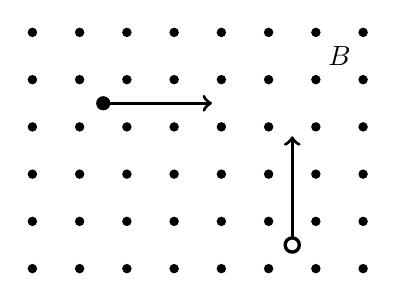
\begin{tikzpicture}[scale=.6]
      \foreach \x in {0,...,7}{
        \foreach \y in {0,...,5} \fill (\x,\y) circle (.1);
      }
      \draw[very thick] (5.5,.5) circle (.15);
      \draw[->,very thick] (5.5,.65)--(5.5,2.8);
      \fill (1.5,3.5) circle (.15);
      \draw[->,very thick] (1.65,3.5)--(3.8,3.5);
      \node at(6.5,4.5){$\bm B$};
    \end{tikzpicture}
  \end{center}
  \begin{enumerate}[itemsep=3pt]
  \item The black circle represents a proton moving to the right. Calculate
    the magnitude and direction of the force on the proton.
  \item The white circle represents an electron moving towards the top of the
    page. Calculate the magnitude and direction of the force on the electron.
  \end{enumerate}

  % Modified from Tipler p.808 Question 31
\item The wire segment in the figure below carries a current of
  $I=\SI{1.8}\ampere$ from $A$ to $B$ to $C$. There is a magnetic field of
  \SI{1.2}{\tesla} coming out of the page. Find the total force on the wire
  and show that it is the same as if the wire were a straight segment from
  $A$ to $C$. Answer to \emph{three} significant figures.
  \begin{center}
    \begin{tikzpicture}[scale=.85]
      \draw[axes] (0,0)--(0,6) node[above]{$y$};
      \draw[axes] (0,0)--(8,0) node[right]{$x$};
      \foreach \x in {.5,1.5,...,7.5} {
        \foreach \y in {.5,1.5,...,5.5} \fill[lightgray] (\x,\y) circle (.08);
      }
      \draw[vectors] (2,1)--(3.6,1)
      node[pos=0,left]{$A$}
      node[below]{\SI3{\centi\metre}}
      node[above]{$I$};
      \draw[very thick] (3.5,1)--(5,1) node[right]{$B$};
      \draw[vectors] (5,1)--(5,3.2) node[right]{\SI4{\centi\metre}};
      \draw[very thick] (5,3)--(5,5) node[right]{$C$};
    \end{tikzpicture}
  \end{center}
\end{enumerate}
